\documentclass[10 pt]{beamer}
\usepackage{color,fancybox,bm}
\usepackage{color}
\usepackage{booktabs}
\usepackage{threeparttable}
\usepackage{dashrule}
\usepackage{float}
\usepackage{graphicx}
\usepackage{amsmath}
\usepackage{fixltx2e}
\usepackage{amssymb}
\usepackage{rotating}
\usepackage{beamerthemeshadow}
\newtheorem{acknowledgement}[theorem]{Acknowledgement}
\newtheorem{algorithm}[theorem]{Algorithm}
\newtheorem{assumption}{Assumption}
\newtheorem{assumption1}{Assumption 1}
\newtheorem{assumptions}{Assumptions}
\newtheorem{axiom}[theorem]{Axiom}
\newtheorem{case}[theorem]{Case}
\newtheorem{thm1}[theorem]{Theorem 1}
\newtheorem{thm2}[theorem]{Theorem 2}
\newtheorem{claim}[theorem]{Claim}
\newtheorem{conclusion}[theorem]{Conclusion}
\newtheorem{condition}[theorem]{Condition}
\newtheorem{conjecture}[theorem]{Conjecture}
\newtheorem{criterion}[theorem]{Criterion}
\newtheorem{exercise}[theorem]{Exercise}
\newtheorem{notation}[theorem]{Notation}
\newtheorem{proposition}[theorem]{Proposition}
\newtheorem{remark}[theorem]{Remark}
\newtheorem{summary}[theorem]{Summary}
\newcommand{\nc}{\newcommand}
\nc{\tr}{\text{tr}}

\useoutertheme{infolines}
\setbeamercolor*{palette
primary}{use=structure,fg=structure.fg,bg=structure.fg!40!white}
\setbeamercolor*{palette
secondary}{use=structure,fg=white,bg=structure.fg!60!white}
\setbeamercolor*{palette
tertiary}{use=structure,fg=white,bg=structure.fg!90!white}
\setbeamercolor*{palette quaternary}{fg=white,bg=black}

\setbeamercolor*{sidebar}{use=structure,bg=structure.fg}

\setbeamercolor*{palette sidebar
primary}{use=structure,fg=structure.fg!10} \setbeamercolor*{palette
sidebar secondary}{fg=white} \setbeamercolor*{palette sidebar
tertiary}{use=structure,fg=structure.fg!50} \setbeamercolor*{palette
sidebar quaternary}{fg=white}

\setbeamercolor*{titlelike}{use=structure,fg=structure.fg,bg=structure.fg!20!white}

\setbeamercolor*{separation line}{} \setbeamercolor*{fine separation
line}{}

\setbeamercolor*{block title example}{fg=black}

\usefonttheme[onlysmall]{structurebold}

\newcommand{\ft}{\frametitle}
\newcommand{\bb}{\begin{block}}
\newcommand{\eb}{\end{block}}
\newcommand{\bi}{\begin{itemize}}
\newcommand{\ei}{\end{itemize}}
\newcommand{\be}{\begin{enumerate}}
\newcommand{\ee}{\end{enumerate}}
\newcommand{\bab}{\begin{alertblock}}
\newcommand{\eab}{\end{alertblock}}
\newcommand{\beb}{\begin{exampleblock}}
\newcommand{\eeb}{\end{exampleblock}}
\newcommand{\bc}{\begin{columns}}
\newcommand{\ec}{\end{columns}}
\newcommand{\ii}{\item}
\newcommand{\convas}{\stackrel{a.s.}{\rightarrow}}
\newcommand{\convp}{\stackrel{p}{\rightarrow}}
\newcommand{\convd}{\stackrel{d}{\rightarrow}}
\newcommand{\ba}{\begin{array}}
\newcommand{\ea}{\end{array}}
\usepackage{ctex}
%\usepackage{jmlr2e}
\usepackage{amsmath}
\newtheorem{myDef}{Definition}
\newtheorem{myTheo}{Theorem}
\newtheorem{myCor}{Corollary}
\newtheorem{myProp}{Proposition}
\usepackage{graphicx}
\usepackage{caption}
\usepackage{AMSFonts}
\usepackage{amsfonts}
\usepackage{subfigure}
\usepackage{listings}
\title[]{NYSE data Analysis}


\author[Shuoli Chen]{Shuoli Chen \\[2mm]}
\institute[]{Institute of Statistics \& Big Data \\ Renmin University of China
	
}

\date{}

\begin{document}
	
	\begin{frame}
	\titlepage
\end{frame}


\begin{frame}
	\begin{itemize}
		\item First we plot the data with timing diagram:
		\begin {figure}[h]
		\centering
		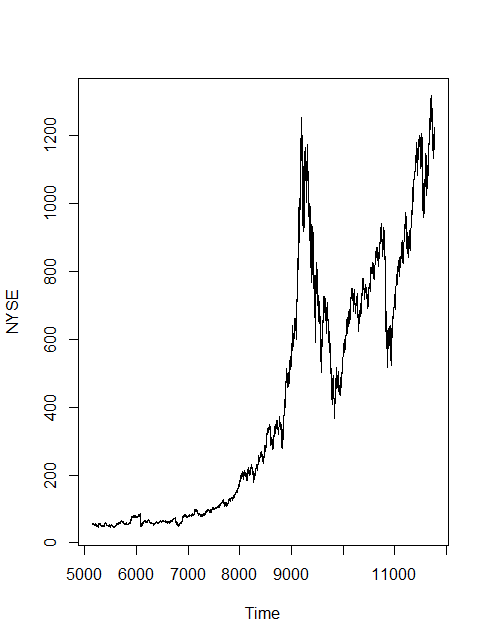
\includegraphics[width=8cm,height=6cm]{NYSE.png}
		\end {figure}
		\item Intuitively, the data is not stationary, not to mention white noise.
	\end{itemize}
\end{frame}



\begin{frame}
	\begin{itemize}
		\item Make the data be stationary with curve-fittin.
		We use $e^{a_0+a_1x+a_2x_2}$ to fit the data, and get the coefficients
		(3.482e+00,    6.837e-04,   -1.793e-08).
		\item We plot the stationary timing diagram:
				\begin {figure}[h]
				\centering
				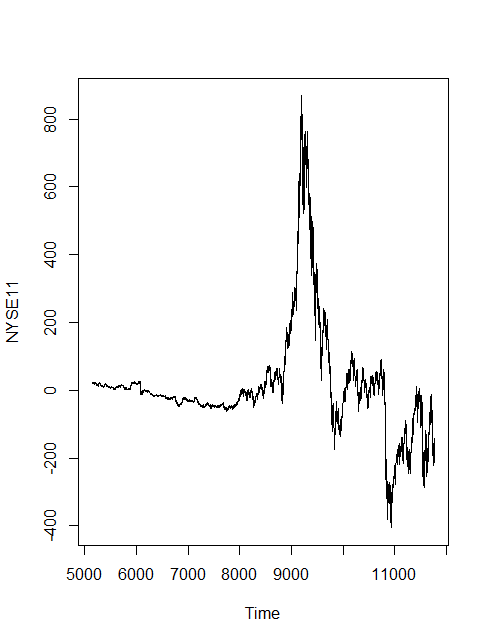
\includegraphics[width=8cm,height=6cm]{NYSE11.png}
				\end {figure}
	\end{itemize}
\end{frame}


\begin{frame}
	\begin{itemize}
		\item 
		We conduct Ljung-Box white noise test to the transformed data and the p-value is 2.2e-16, so we can see that the transformed data is significantly not white noise.
		\item we check if the transformed data is stationary with adf test, the p-value is 0.5184, so the transformed data is stationary
		\item Obviously there is ARCH effect in the data. First, we can routinely build a linear time series model, for example the ARMA model. Then we consider to construct an appropriate ARCH model for the residue.
	\end{itemize}
\end{frame}

\begin{frame}


\begin{itemize}
	\item Build an ARMA model.\\
	The notation ARMA $(p, q)$ refers to the model with $p$ autoregressive terms and $q$ moving-average terms. 
    \item This model contains the $A R(p)$ and $M A(q)$ models
	\[
	X_{t}=c+\varepsilon_{t}+\sum_{i=1}^{p} \varphi_{i} X_{t-i}+\sum_{i=1}^{q} \theta_{i} \varepsilon_{t-i}
	\]\\
	$\mu$ is the expectation of $X_{t}$ (often assumed to equal 0), and the $\{\epsilon_t\}$ are white noise error terms.
\end{itemize}
\end{frame}


\begin{frame}
	
	\begin{itemize}
		\item ARMA(5,4) is the best model according to the corresponding AIC values. The coefficients are $\psi = (-0.48, -0.58, 0.605, 0.495), \theta = (0.952, 1.491, 2.05, 1.43, 0.945), c = 14.71.$
		
		\item Box-Ljung test shows the residual of ARMA(5,4) model is white noise, significance test shows the coefficients of ARMA(5,4) are significant. 

	\end{itemize}
\end{frame}


\begin{frame}
	
	
	\begin{itemize}
		\item We plot the ARMA residuals with timing diagram:
		\begin {figure}[h]
		\centering
		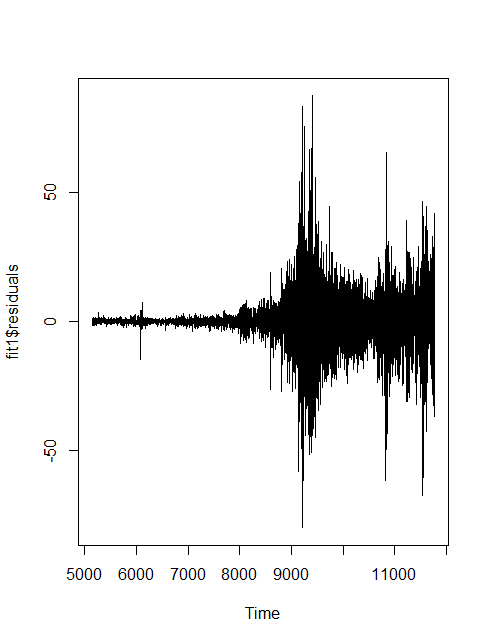
\includegraphics[width=8cm,height=6cm]{NYSE_res1.png}
		\end {figure}
		\item Obviously we can observe the ARCH effect, so we need to build a model for the residuals of ARMA(5,4).
		
	\end{itemize}
\end{frame}




\begin{frame}


\begin{itemize}
	\item ARCH model:
	
	Assume $\epsilon_{t}=\sigma_{t} z_{t},$ where $z_{t} \overset{iid}\sim  N(0,1)$, The model of $\sigma_{t}$ is
	$\sigma_{t}^{2}=\alpha_{0}+\alpha_{1} \varepsilon_{t-1}^{2}+\cdots+\alpha_{p} \varepsilon_{t-p}^{2}.$
	
	\item If we apply the idea of ARMA to model $\sigma_{t}^{2}$, we get GARCH model:
	$\sigma_{t}^{2}=\alpha_{0}+\alpha_{1} \varepsilon_{t-1}^{2}+\cdots+\alpha_{q} \varepsilon_{t-q}^{2}+\beta_{1} \sigma_{t-1}^{2}+\cdots+\beta_{p} \sigma_{t-p}^{2}.$
	\item We consider GARCH model. In fact, GARCH(1,1) is simple and efficient. The cofficients of GARCH(1,1) are
	$\alpha_0 = 0.007149, \alpha_1 = 0.099418, \beta_1 =  0.907365.$
	
\end{itemize}
\end{frame}


\begin{frame}
	
	
	\begin{itemize}

		\item Box-Ljung test shows the residual of ARMA(5,4) model is white noise, significance test shows the coefficients of ARMA(5,4) are significant.
		\item We plot the GARCH residuals:
		\begin {figure}[h]
		\centering
		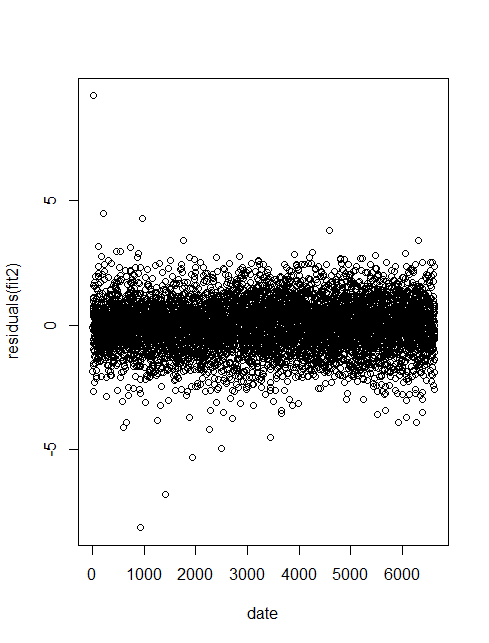
\includegraphics[width=8cm,height=6cm]{NYSE_res2.png}
		\end {figure}
		\item According to the figure, we can see that there is no ARCH effect in GARCH residual. Hence GARCH(1,1) model is predictive to the risk of stock market. With GARCH(1,1) we can predict when high risk happens and then avoid it.
		
	\end{itemize}
\end{frame}

\begin{frame}
	
	
	\begin{itemize}
\item In fact, it is not every GARCH(p,q) that works well, for example, the residuals of GARCH(2,2) model is
\begin {figure}[h]
\centering
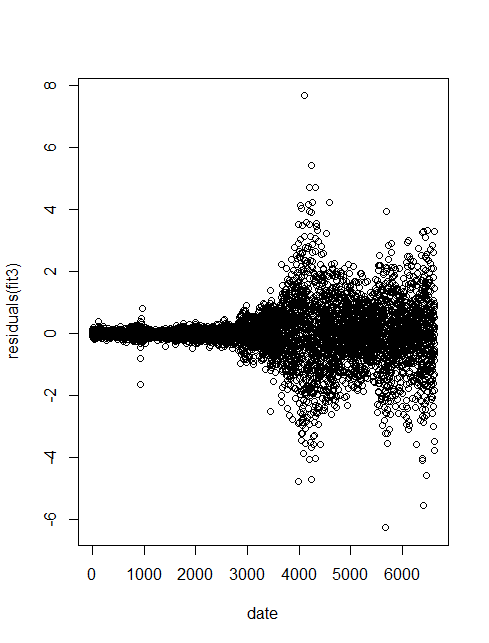
\includegraphics[width=8cm,height=6cm]{NYSE_res3.png}
\end {figure}
\item It is obvious that there is ARCH effect in residual of GARCH(2,2), hence GARCH(2,2) can not help us to avoid high risk in stock exchange.
	\end{itemize}
\end{frame}

\end{document}

